\section{Matriz SWOT}

A matriz SWOT, também conhecida como matriz FOFA, é uma ferramenta gerencial que examina o ambiente interno e externo de uma organização, buscando identificar as as suas forças, fraquezas, oportunidades e ameaças, para encontrar oportunidades de melhoria e otimização do desempenho\cite{santella_MatrizSWOT_blog2020}.

A figura \ref{fig:matrizSWOT} apresenta a matriz SWOT, com a análise desses quatro elementos de acordo com o contexto do projeto proposto.

\begin{figure}[H]
  \centering
  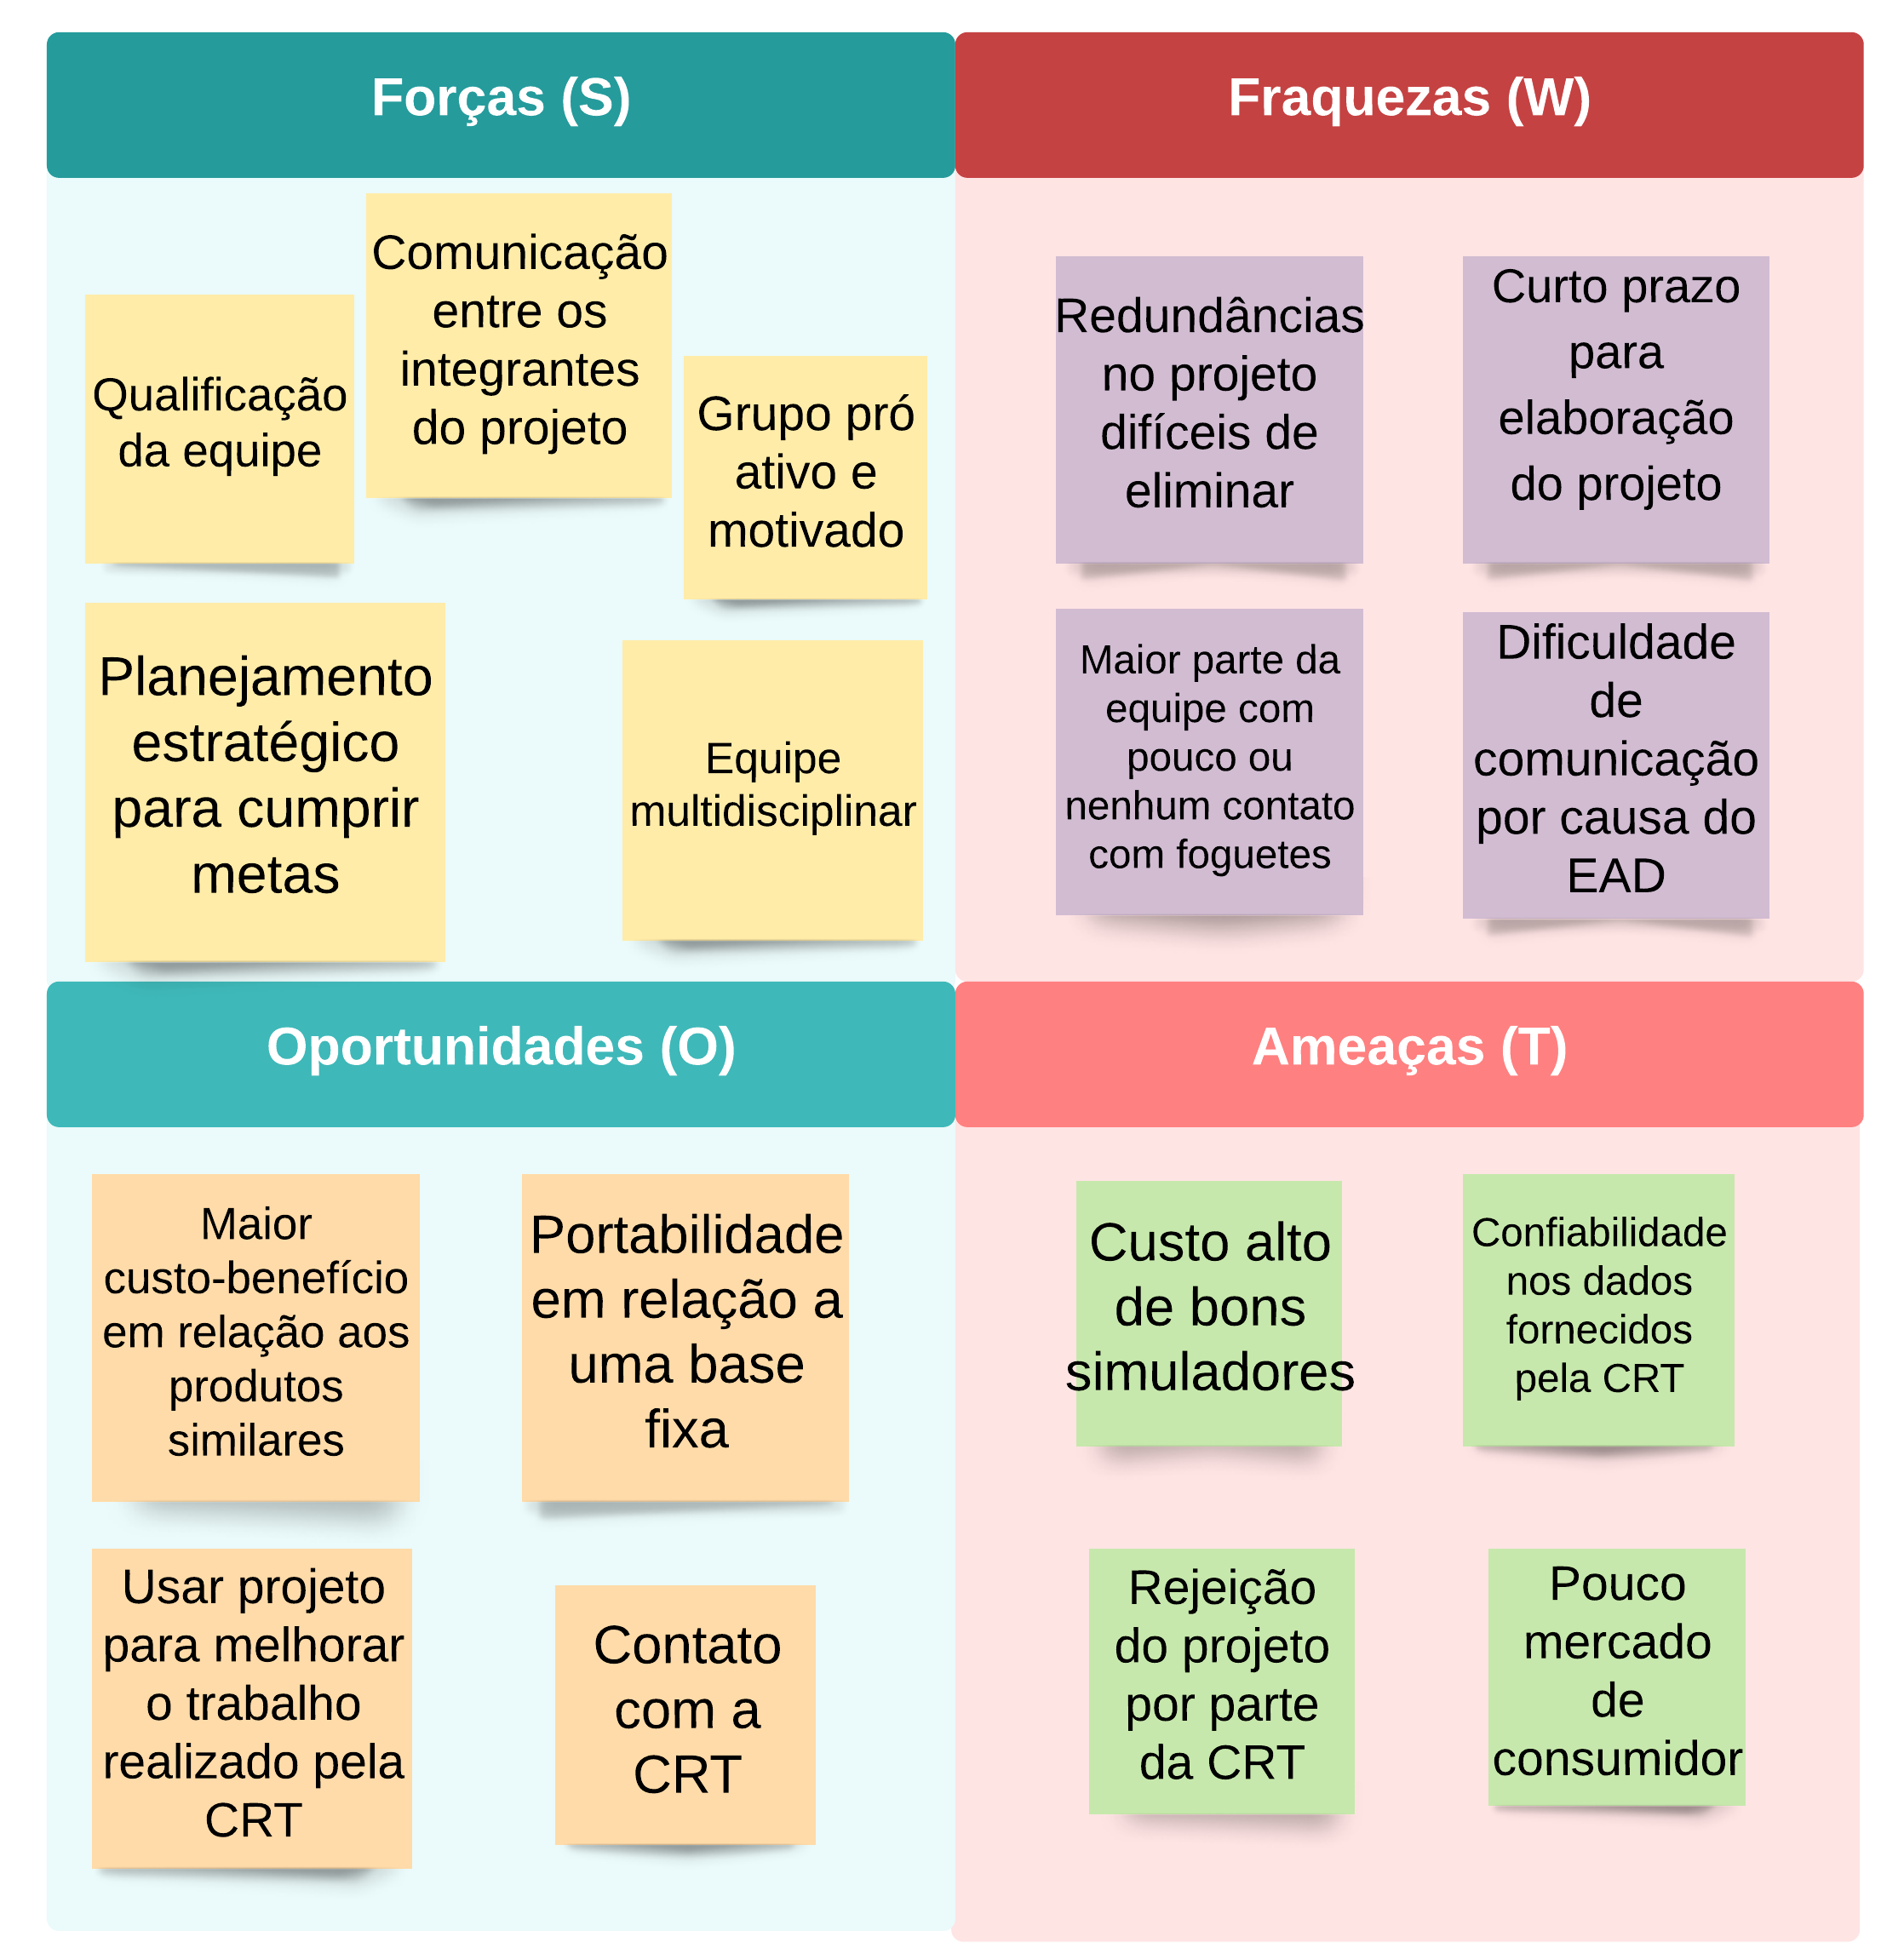
\includegraphics[scale=0.15]{figuras/SWOT_BaseLancamento.png}
  \caption{Matriz \textit{SWOT}. Matriz foi construída usando a ferramenta Lucidchart.} 
  \label{fig:matrizSWOT}
\end{figure}